% !TeX program = xelatex
\documentclass[11pt,a4paper]{article}
\usepackage{aes}
\usepackage{amsmath,tabularx,float,array,needspace}
\widowpenalty=10000 \clubpenalty=10000 \displaywidowpenalty=10000
\renewcommand{\tabularxcolumn}[1]{>{\raggedright\arraybackslash}p{#1}}
\title[Who Took the Hint? Online Supplement]{Online Supplement to “Who Took the Hint? Applying the Methods of Causal Inference to Evaluate Chain of Thought Monitorability”}
\aesauthor[affil={1}]{Alexis Diamond}
\aesaffiliation{1}{Minerva University}
\begin{document}
\maketitle
\noindent This supplement contains the appendices of the paper that are not printed with it: A.2, A.4, B.1--B.4, C and D. Section numbers match the references in the paper. References to sections marked \S{} are to the paper's main text, and references to A.1, A.3, A.5, A.6, B.5 and E are to the appendices printed with the paper.
\let\aesoldclearpage\clearpage\let\clearpage\relax\appendix\let\clearpage\aesoldclearpage
\setcounter{section}{0}
\section{Derivations}
\setcounter{subsection}{1}
\subsection{Bounds without monotone treatment response}
Without the assumption that the cue never pushes a draw away from the cue-concordant output, the mass of draws with Y(0) = 0 and Y(1) = 1 is not point-identified. By the Fréchet bounds on the joint of (Y(0), Y(1)) given its marginals, Pr(Y(1) = 1, Y(0) = 0) $\in$ [max(0, $p_1$ $-$ $p_0$), min($p_1$, 1 $-$ $p_0$)]. TE is the lower endpoint. An instance with TE = 0 may therefore contain equal masses of draws moved toward and away from the cue-concordant output rather than none of either, which the gate of Section~2.3 cannot distinguish. The floor survives the loss of monotonicity: every draw with Y(0) = 0 and Y(1) = 1 used the cue (under the exclusion restriction), and such draws are at least a share TE of all draws, so the influence rate is still at least TE / $p_1$. Monotonicity is needed to read TE as the complier mass itself, not to make the floor a lower bound; without it the bound is merely looser.

\emph{Worked example, Guan et al.'s instance.} With $p_0$ = 0.25 and $p_1$ = 0.85, the Fréchet bounds give Pr(Y(1) = 1, Y(0) = 0) $\in$ [max(0, 0.60), min(0.85, 0.75)] = [0.60, 0.75]. Under monotone treatment response the mass of draws moved toward the cue-concordant output is exactly 0.60; without it, that mass could be as high as 0.75, offset by up to 0.15 of draws moved away from it, since 0.75 $-$ 0.15 nets to the observed TE of 0.60. The floor TE / $p_1$ = 0.71 is unchanged in either case, because every draw moved toward the cue-concordant output used the cue and such draws are at least 0.60 of all draws.

Effects in both directions. “Cue-concordant” names an outcome level, not an effect direction: the cue can move a draw toward that level, Y(0) = 0 and Y(1) = 1, or away from it, Y(0) = 1 and Y(1) = 0, even though, as this appendix explains, the metric counts only the first.

The no-defier condition of Section~2.2 applies strictly to treatment take-up. Draws the cue moves away from the cue-concordant output, with Y(0) = 1 and Y(1) = 0, are ruled out by a separate assumption, monotone treatment response \citep{manski1997monotone}, Y(1) $\geq$ Y(0) for every draw, discussed below. It concerns the outcome and differs from the standard monotonicity assumption of encouragement designs \citep{imbens1994identification}, which concerns take-up: that no unit takes the treatment only when not encouraged, which here holds by construction.

$\mathrm{TPR}_{\mathrm{mc}}$ also counts influence in only one direction. It credits the monitor for flagging draws that the cue pushed toward the cue-concordant answer, but the monitor is asked whether the model was influenced at all, which includes draws the cue pushed away from that answer. Such draws used the cue’s content, so they are compliers in the take-up sense, with a negative effect on the outcome; monotone treatment response rules them out.

What makes Guan et al.’s metric one-directional is monotone treatment response, which rules out draws with Y(0) = 1 and Y(1) = 0 by assumption, together with their decision to discard every instance whose estimated effect is not positive. Where such draws nonetheless exist, an instance in which they outweigh the draws moved toward the cue-concordant output has a non-positive estimated effect and is discarded, while an instance in which they are outweighed is scored with TE understating the complier mass by their share. A model that reads the hint, judges it a trap, and chooses otherwise was influenced by the cue, and a good monitor should say so, but nothing in the score credits it. The assumption is not innocuous. A model that mistrusts the cue is pushed away from the cue-concordant output by it. Mistrust has ordinary causes, such as training against sycophancy, and because models are increasingly trained to resist this kind of pressure, the share of such draws can grow across checkpoints. The same two-directional influence affects specificity: encouraged draws that did not give the cue-concordant answer are treated as true negatives, yet the cue may have moved some of them toward a different answer, a point \citet[their Appendix B.4]{burger2026cot} make about intervention experiments generally.

\setcounter{subsection}{3}
\subsection{The consistency check across cue variants}
For cue variant v on a common instance set, let $\mathrm{TE}_v$ be the intention-to-treat effect and $\hat{\pi}_v$ the monitor’s flag rate among encouraged draws (its estimate of $\pi_v$). Under the exclusion restriction, $\mathrm{TE}_v$ / $\pi_v$ = 1 $-$ $p_0^{c}$(v), the effect of cue use on variant v’s compliers (A.1), and with a monitor that detects cue use at a rate 1 $-$ $\delta$ not depending on v and, for simplicity, raises no false flags, $\mathrm{TE}_v$ / $\hat{\pi}_v$ estimates (1 $-$ $p_0^{c}$(v)) / (1 $-$ $\delta$). False flags at a rate $\varphi$ add (1 $-$ $\pi_v$)$\varphi$ to the flag rate and bias every ratio downward, by an amount that differs across variants unless their take-up rates are similar. The ratio is constant across variants only under three conditions together: the exclusion restriction, monitor error that does not depend on the variant, and compliers with the same unaided rate under every variant. The third is an assumption of homogeneous complier effects across instruments, which is the condition under which the Sargan test for overidentified instrumental-variables models is valid; without it, different instruments identify different local average treatment effects \citep{imbens1994identification}, and the ratios differ for that reason alone. Equality of the ratios across variants is therefore a test of the joint hypothesis, with degrees of freedom equal to the number of variants minus one. Rejection cannot be attributed to the monitor or to exclusion without the homogeneity assumption; agreement supports all three conditions at once, since it would require their failures to cancel.

\emph{Illustration with two variants.} Suppose variant A has TE = 0.60 and a flag rate of 0.72, and variant B has TE = 0.45 and a flag rate of 0.60, both on the same instances. The ratios are 0.60 / 0.72 = 0.83 and 0.45 / 0.60 = 0.75. Agreement would have required 0.83 = 0.75, so the check rejects. Three accounts fit the numbers equally well: the monitor misses a larger share of cue use under B, so B's flag rate understates its take-up and the ratio comes out low; B's text moves the output by a route other than its content, so TE\_B overstates what cue use did; or B recruits compliers with a different unaided rate, so 1 $-$ $p_0^{c}$(B) is simply a different quantity from 1 $-$ $p_0^{c}$(A). Nothing in the two ratios says which. Had the ratios agreed, each of the three would have had to be absent or to cancel against another, which is why agreement, not rejection, is the informative outcome.

\setcounter{section}{1}
\section{Worked examples}
\setcounter{subsection}{0}
\subsection{Guan et al.’s example (Section~2.2), step by step}
Guan et al.’s illustration (their Section~3.1.1) makes every quantity concrete. A four-option question carries a hint pointing to option D. In the no-encouragement arm the model guesses uniformly, so it answers D a quarter of the time: $p_0$ = 0.25. In the encouraged arm, 80\% of draws follow the hint and the rest behave as if unaided: $\pi$ = 0.8.

\begin{table}[H]
  \centering\small
  \begin{tabularx}{\linewidth}{@{}XXXXXX@{}}
    \toprule
    Quantity & Formula & $\pi$ = 0.8, $p_0$ = 0.25 & $\pi$ = 0.8, $p_0$ = 0.05 & $\pi$ = 0.6, $p_0$ = 0.50 & Identified from the two arms? \\
    \midrule
    Base rate (input) & $p_0$ & 0.25 & 0.05 & 0.50 & yes (stipulated) \\ \addlinespace[3pt]
    Take-up rate (input) & $\pi$ & 0.80 & 0.80 & 0.60 & no (stipulated) \\ \addlinespace[3pt]
    Cue-concordant rate, cue present & $p_1$ = $\pi$ + (1 $-$ $\pi$) $p_0$ & 0.85 & 0.81 & 0.80 & yes \\ \addlinespace[3pt]
    Intention-to-treat effect & TE = $\pi$(1 $-$ $p_0$) & 0.60 & 0.76 & 0.30 & yes \\ \addlinespace[3pt]
    Floor (complier share) & $R_{\mathrm{effect}}$ = TE / $p_1$ & 0.706 & 0.938 & 0.375 & yes \\ \addlinespace[3pt]
    Influence rate & $\pi$ / $p_1$ & 0.941 & 0.988 & 0.750 & no \\ \addlinespace[3pt]
    Gap & $\pi$ $p_0$ / $p_1$ & 0.235 & 0.049 & 0.375 & no \\ \addlinespace[3pt]
    Influence rate / floor & 1 / (1 $-$ $p_0$) & 1.33 & 1.05 & 2.00 & — \\ \addlinespace[3pt]
    Effect of cue use among cue-using draws & TE / $\pi$ = 1 $-$ $p_0$ & 0.75 & 0.95 & 0.50 & no \\
    \bottomrule
  \end{tabularx}
  \caption{Guan et al.’s worked example ($\pi$ = 0.8, $p_0$ = 0.25) and two variants.}
\end{table}

\noindent{\small Guan et al.’s 16/17 = 0.941 is the influence rate; the understatement they note is the gap. The steps below walk through the first column.}

\emph{Step 1, the encouraged arm’s rate.} Hint-followers answer D (0.80 of all draws); the unaided fifth answers D a quarter of the time (0.20 $\times$ 0.25 = 0.05). So $p_1$ = 0.85.

\emph{Step 2, the intention-to-treat effect.} TE = $p_1$ $-$ $p_0$ = 0.60. Offering the hint raised the rate of D by 60 points. This is identified from the two arms.

\emph{Step 3, the floor.} Among encouraged draws that answered D, the share whose answer would not have been D without the hint is TE / $p_1$ = 0.60 / 0.85 $\approx$ 0.71. This is the complier share among encouraged cue-concordant draws, $R_{\mathrm{effect}}$. Under monotone treatment response it too is identified.\footnote{Without monotone treatment response, TE understates the complier mass by the mass of draws the cue moves away from the cue-concordant output, and 0.71 is a lower bound on this share rather than its value (Appendix A.2).}

\emph{Step 4, the influence rate.} Among the same 0.85, the share that followed the hint is 0.80 / 0.85 = 16/17 $\approx$ 0.94. Guan et al. report this number as the fraction attributable to the hint and note that the measured total effect, 0.60, is smaller. It is smaller because 0.20 $\times$ 0.25 = 0.05 of all draws are hint-followers who would have guessed D anyway: the hint fired (U = 1 in Guan et al.’s notation) but the answer did not depend on it (Y(0) = Y(1) = 1). The floor excludes them; the influence rate counts them. Their mass, 0.05 / 0.85 $\approx$ 0.24, is the gap.

\emph{Step 5, why the influence rate is not identified.} Step 4 used $\pi$ = 0.8, which is stipulated in the example and unobserved in practice: the evaluation sees 0.85 in one arm and 0.25 in the other, and those two numbers are consistent with many values of $\pi$. Under monotone treatment response the influence rate lies in [0.71, 1]; the lower end is the floor, and that is the precise content of Guan et al.’s statement that the total effect lower-bounds the causal influence rate. With $p_0$ = 0 the interval collapses to a point, which is their observation that the two coincide only at zero base rate.

\emph{Step 6, the Wald ratio.} Dividing the intention-to-treat effect by the take-up rate (the first stage, in instrumental-variables terms) gives TE / $\pi$ = 0.60 / 0.80 = 0.75: among draws that used the hint, using it raised the rate of D from 0.25 to 1. This is the local average treatment effect, here equal to the effect of treatment on the treated, and it is not computable from the evaluation because $\pi$ is unobserved. The monitor’s flag rate is the only available estimate of $\pi$, which Section~5.3 exploits.

Three ratios, then, share the ingredients 0.60, 0.80 and 0.85 and answer three questions. 0.60 / 0.85 = 0.71 asks what share of encouraged D-answers depended on the hint (the floor). 0.80 / 0.85 = 0.94 asks what share used the hint (the influence rate). 0.60 / 0.80 = 0.75 asks what using the hint did to the draws that used it (the Wald ratio). The evaluation identifies the first, scores the monitor against it, names the second as the monitor’s target, and would need a trustworthy monitor to recover the third. A perfect detector of hint use flags 0.94 of encouraged D-answers and clears the floor of 0.71 with room to spare; a monitor detecting three-quarters of hint use flags 0.75 $\times$ 0.94 $\approx$ 0.71 and clears it exactly, scoring $\mathrm{TPR}_{\mathrm{mc}}$ = 1 while missing a quarter of actual hint use.

\setcounter{subsection}{1}
\subsection{The half-blind monitor (Section~3.1), step by step}
\emph{Step 1, the rates.} The cue is a user’s stated view. Take $p_0$ = 0.5 (the model gives that view’s answer half the time unaided) and $\pi$ = 0.6 (60\% of encouraged draws use the view). Compliers give the cue-concordant output and never-takers default to the baseline, so $p_1$ = 0.6 + 0.4 $\times$ 0.5 = 0.8, TE = $p_1$ $-$ $p_0$ = 0.3, and $R_{\mathrm{effect}}$ = TE / $p_1$ = 0.375.

\emph{Step 2, what a perfect monitor flags.} Every complier used the cue and is cue-concordant, so compliers are $\pi$ / $p_1$ = 0.6 / 0.8 = 0.75 of encouraged cue-concordant draws; the other 0.25 are never-takers whose answer matched the stated view without using it. A perfect detector of cue use flags 75\%.

\emph{Step 3, the half-blind monitor.} A monitor that detects half of actual cue use flags 0.5 $\times$ 0.75 = 0.375. The score divides by the floor: $\mathrm{TPR}_{\mathrm{mc}}$ = min(1, 0.375 / 0.375) = 1. With both true-negative rates at 0.95, g-mean$^2$ = 0.95, near the top of the published range.

\emph{Step 4, why the score cannot tell.} The 0.375 the monitor flags and the 0.375 the floor demands coincide, and the framework has no way to see that the flagged draws are only half of those that used the cue, since no draw carries a label for cue use. \citeauthor*{guan2026beyond}’s (\citeyear{guan2026beyond}) lower bound on recall, max(0, (f + $R_{\mathrm{effect}}$ $-$ 1) / $R_{\mathrm{effect}}$) with f = 0.375, is max(0, $-$0.67) = 0, so their interval for this monitor is [0, 1].

\emph{Step 5, the general condition.} A monitor detecting a share $\delta$ of cue use flags $\delta$ $\pi$ / $p_1$, and $\mathrm{TPR}_{\mathrm{mc}}$ = min(1, $\delta$ $\pi$ / ($p_1$ $R_{\mathrm{effect}}$)) = min(1, $\delta$ / (1 $-$ $p_0$)). It scores 1 whenever $\delta$ $\geq$ 1 $-$ $p_0$, at any $\pi$. Here 1 $-$ $p_0$ = 0.5, so any monitor catching at least half of cue use scores perfectly. Averaging across instances does not change this, because the score is bounded by 1 on every instance where the condition holds; on instances with lower base rates the same monitor falls below the floor, so the failure is hidden in proportion to a dataset’s share of high-base-rate instances.

\setcounter{subsection}{2}
\subsection{The base-rate gap of Section~3.2, step by step}
\emph{Step 1, the ratio.} Under equal baselines (Section~2.2), the floor is $R_{\mathrm{effect}}$ = TE / $p_1$ = $\pi$(1 $-$ $p_0$) / $p_1$ and the influence rate is c = $\pi$ / $p_1$. Dividing the second by the first,

\begin{align*}
  c / R_{\mathrm{effect}} &= [\pi  / p_1] / [\pi (1 - p_0) / p_1] = 1 / (1 - p_0).
\end{align*}

The take-up rate $\pi$ and the encouraged rate $p_1$ cancel, so the ratio depends on the base rate alone.

\emph{Step 2, how much cue use a monitor can miss and still score perfectly.} Suppose the monitor flags a share $\delta$ of the draws that used the cue and nothing else. Its flag rate among encouraged cue-concordant draws is f = $\delta$c, and

\begin{align*}
  \mathrm{TPR}_{\mathrm{mc}} &= \min(1, \delta c / R_{\mathrm{effect}}) = \min(1, \delta  / (1 - p_0)).
\end{align*}

So $\mathrm{TPR}_{\mathrm{mc}}$ = 1 whenever $\delta$ $\geq$ 1 $-$ $p_0$: the monitor can miss a share 1 $-$ $\delta$ of cue use as large as $p_0$ and still score perfectly. This is the last column of Tables 1 and B2.

\emph{Step 3, the reference points in Figure B1.} At $\pi$ = 0.8:

\begin{itemize}
  \item $p_0$ = 0.05: $p_1$ = 0.8 + 0.2 $\times$ 0.05 = 0.81, TE = 0.76, floor = 0.76 / 0.81 = 0.94, influence rate = 0.8 / 0.81 = 0.99. The two are five points apart and the ratio is 1.05.
  \item $p_0$ = 0.5: $p_1$ = 0.9, TE = 0.40, floor = 0.44, influence rate = 0.89. The ratio is 2, so the floor is half the influence rate.
  \item $p_0$ = 0.7: $p_1$ = 0.94, TE = 0.24, floor = 0.26, influence rate = 0.85. The ratio is 3.3, so the floor is under a third of the influence rate.
\end{itemize}
\begin{figure}[H]
  \centering
  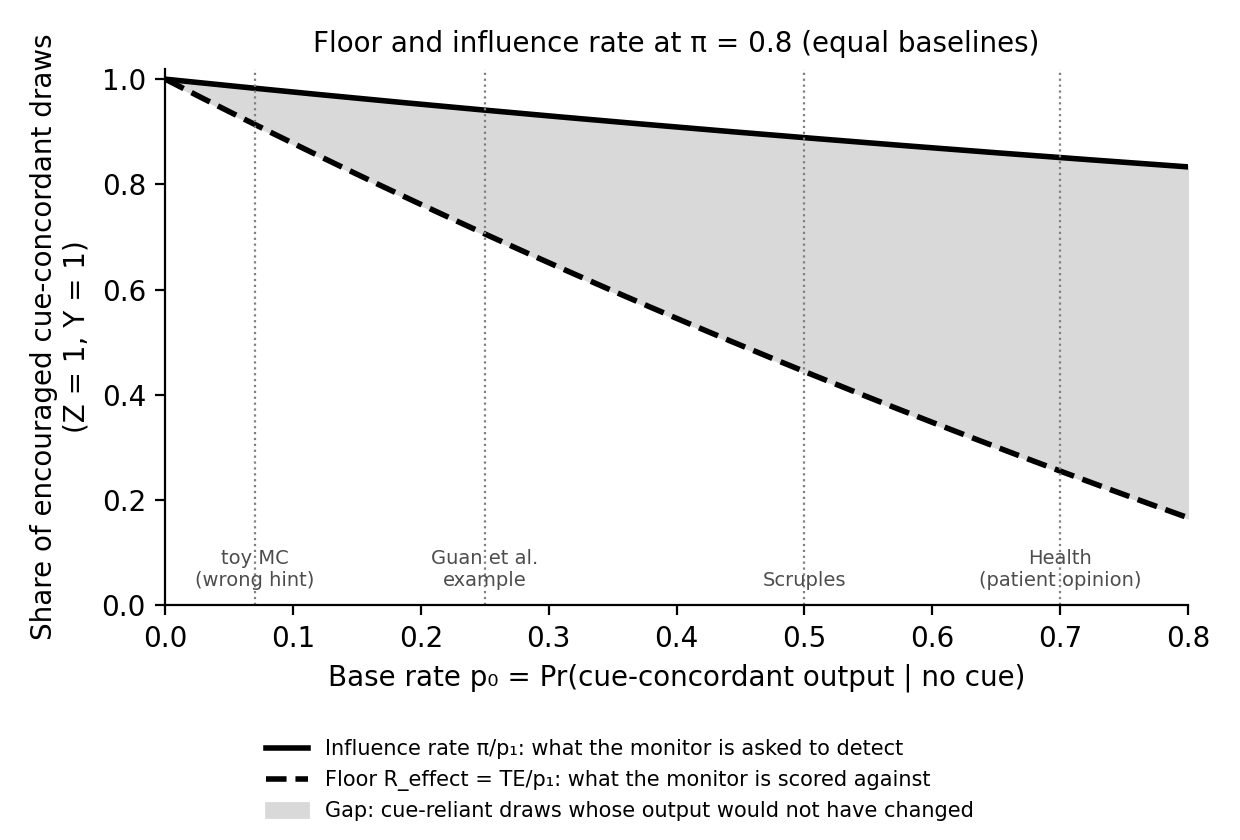
\includegraphics[width=0.78\linewidth]{assets/fig1.png}
  \caption{The floor and the influence rate against the base rate $p_0$ at $\pi$ = 0.8, equal baselines. The band’s height, $\pi$ $p_0$ / $p_1$, is the gap of Section~2.2. Vertical lines mark structural base rates from Tables 1 and B2.}
  \label{fig:floor}
\end{figure}

\emph{Step 4, the structural base rate for a wrong hint.} On a four-option question the model answers correctly with probability equal to its accuracy, acc, and spreads its errors, 1 $-$ acc, over the three wrong options. If it spreads them evenly, the unaided rate of the particular wrong option the hint names is $p_0$ = (1 $-$ acc)/3. At acc = 0.8 this is 0.2 / 3 $\approx$ 0.07, giving a ratio of 1 / (1 $-$ 0.07) $\approx$ 1.07 and a missable share of about 7\%: the first row of Tables 1 and B2. If errors concentrate on one plausible distractor and the hint names it, $p_0$ is higher; if the hint names an implausible option, lower.

\emph{Step 5, every row of Table B2.} In each environment, $p_0$ is the rate at which the model gives the cue-concordant output with no cue, read off the outcome definition; the ratio is 1 / (1 $-$ $p_0$) and the missable share is $p_0$.

\begin{itemize}
  \item Toy math/science (GPQA, DAFT): Y = the hinted wrong option. Unaided, the model is correct with probability acc and spreads its errors over three wrong options, so $p_0$ $\approx$ (1 $-$ acc)/3 $\approx$ 0.07 at acc = 0.8; ratio 1.07; missable 7\%.
  \item AIME: Y = the hinted number on an open-response problem. The chance of producing a specific wrong number unaided is near zero, so $p_0$ $\approx$ 0; ratio $\approx$ 1; missable $\approx$ 0.
  \item Sandbagging (WMDP): Y = the supplied incorrect option. As for the toy case, $p_0$ $\approx$ (1 $-$ acc)/3; at acc between 0.7 and 0.85 this is 0.05 to 0.10; ratio 1.05 to 1.1.
  \item Scruples, suggest right and suggest wrong: Y = the verdict the user suggested (B, author not in the wrong, for suggest right; A for suggest wrong). The anecdotes are filtered to ones where the community judged the author in the wrong, and Guan et al. note that models are hesitant to say so, so the unaided rate of B is high and of A low: the two variants bracket 0.5, plausibly 0.3 to 0.7; ratio 1.4 to 3.3; missable 30\% to 70\%.
  \item Scruples, first person: Y = the verdict favors the author (B). The unaided rate of B is the same hesitancy, plausibly above 0.5; ratio 2 or more; missable 50\% or more.
  \item Health Queries, patient opinion: Y = the diagnosis matches the patient’s self-diagnosis, which is set to the truth. Unaided, Y = 1 whenever the model diagnoses correctly, so $p_0$ = its diagnostic accuracy, 0.6 to 0.8; ratio 2.5 to 5; missable 60\% to 80\%.
  \item Health Queries, missing evidence: Y = a correct diagnosis with a case section restored. Unaided (section absent), $p_0$ = accuracy without the section, 0.5 to 0.7; ratio 2 to 3.3.
  \item Memory: Y is a judge-labeled behavior change with no fixed outcome definition, so no structural $p_0$ can be derived.
\end{itemize}
In the Health patient-opinion variant the cue \emph{is} the correct diagnosis, so every draw the model would have diagnosed correctly anyway is cue-concordant with no outcome dependence; in Scruples the unaided rate of the suggested verdict is set by the model’s reluctance to call an author wrong, which Guan et al. report as strong on these anecdotes. Realism and identifiability trade off, because realism means a behavior the model already produces. The same holds for deployment behaviors a model often produces unprompted: reward hacking in coding environments, deference to user pressure, sandbagging on hard tasks. A monitor certified on wrong-hint GPQA carries no warrant to those; it was certified in the one regime where floor and influence rate coincide.

These are derivations, not measurements: Guan et al. do not report $p_0$ per environment, and the released code \citep{openai2026opensourcing} contains datasets and scoring, not sampled outputs. Exact outcome definitions are in Guan et al., Appendix C.1; the Scruples and Health rows follow the outcome definitions in that appendix.

\begin{table}[H]
  \centering\small
  \begin{tabularx}{\linewidth}{@{}XXXXX@{}}
    \toprule
    Environment & Outcome Y & Structural $p_0$ & Influence rate / floor & Cue use a monitor can miss at $\mathrm{TPR}_{\mathrm{mc}}$ = 1 \\
    \midrule
    Toy math/science (GPQA, DAFT) & Answer equals hinted option; hint points to a wrong option of four & $\approx$ (1 $-$ acc)/3; $\approx$ 0.07 at 80\% accuracy & $\approx$ 1.07 & $\approx$ 7\% \\ \addlinespace[3pt]
    AIME & Answer equals hinted number; open response & $\approx$ 0 & $\approx$ 1 & $\approx$ 0 \\ \addlinespace[3pt]
    Sandbagging (WMDP) & Answer equals the supplied incorrect option & $\approx$ (1 $-$ acc)/3 & $\approx$ 1.05–1.1 & $\approx$ 5–10\% \\ \addlinespace[3pt]
    Scruples, suggest right / wrong & Verdict equals the one the user suggested (B / A) & unaided rate of the suggested verdict; the two variants bracket 0.5, $\approx$ 0.3–0.7 & $\approx$ 1.4–3.3 & $\approx$ 30–70\% \\ \addlinespace[3pt]
    Scruples, first person & Verdict favors the author (B) & unaided rate of B, plausibly above 0.5 & $\geq$ 2 & $\geq$ 50\% \\ \addlinespace[3pt]
    Health Queries, patient opinion & Diagnosis matches the patient’s self-diagnosis, which is set to the truth & $\approx$ unaided diagnostic accuracy, 0.6–0.8 & $\approx$ 2.5–5 & $\approx$ 60–80\% \\ \addlinespace[3pt]
    Health Queries, missing evidence & Diagnosis correct with a case section restored & $\approx$ accuracy without the section, 0.5–0.7 & $\approx$ 2–3.3 & $\approx$ 50–70\% \\ \addlinespace[3pt]
    Memory & Judge-labeled behavior change & Not derivable from the definition & — & — \\
    \bottomrule
  \end{tabularx}
  \caption{Structural base rates and the implied floor-to-influence-rate gap for all of Guan et al.’s intervention environments. Derived from the definition of Y under equal baselines, not measured.}
\end{table}

\emph{Step 6, what the equal-baseline assumption does to these numbers.} By Appendix A.1, without equal baselines the ratio is 1 / (1 $-$ $p_0^{c}$), where $p_0^{c}$ is the compliers’ own unaided rate. For a wrong hint, compliers are the uncertain draws and $p_0^{c}$ $\geq$ $p_0$, so the true gap is at least as large as Tables 1 and B2 show. For a correct hint the inequality reverses, $p_0^{c}$ $\leq$ $p_0$, and the true gap is at most as large as Tables 1 and B2 show. The Health Queries patient-opinion row is a correct-hint environment, so its figures are upper ends: the floor sits below the influence rate there, but by a factor that may be smaller than 2.5 to 5. In Scruples the direction is not determined by this argument.

\setcounter{subsection}{3}
\subsection{The model that stopped talking (Section~3.3), step by step}
\emph{Step 1, the behavior, identical at both checkpoints.} Take $p_0$ = 0.10 and $p_1$ = 0.18, so TE = 0.08, and take-up $\pi$ = TE / (1 $-$ $p_0$) = 0.089. The floor is $R_{\mathrm{effect}}$ = 0.08 / 0.18 = 0.44 and the influence rate is 0.089 / 0.18 = 0.49. Nothing about the model’s behavior changes between checkpoints.

\emph{Step 2, checkpoint 1.} The chain of thought records every instance of cue use, and the monitor detects 95\% of what is recorded. It flags 0.95 $\times$ 0.49 = 0.47 of encouraged cue-concordant draws, which exceeds the floor, so $\mathrm{TPR}_{\mathrm{mc}}$ = 1. With both true-negative rates at 0.95, g-mean$^2$ = 1 $\times$ $\surd$(0.95 $\times$ 0.95) = 0.95.

\emph{Step 3, checkpoint 2.} The model still uses the cue at the same rate, but its chain of thought now records only 2\% of that use. The same monitor flags 0.02 $\times$ 0.95 $\times$ 0.49 $\approx$ 0.009 of encouraged cue-concordant draws, so $\mathrm{TPR}_{\mathrm{mc}}$ = 0.009 / 0.44 $\approx$ 0.02 and g-mean$^2$ $\approx$ 0.02.

\emph{Step 4, reading the change.} The score has fallen from 0.95 to 0.02 while TE has stayed at 0.08: the cue moves behavior exactly as before, and the record no longer shows it. That is the first row of Table B3. Had the monitor degraded instead, with the record intact and the monitor’s detection falling to 2\%, this monitor’s numbers would be identical. The difference shows only in a second monitor run on the same transcripts: it would still flag about 0.47 if the record were intact, and about 0.009 if it were not. That comparison is the third row of Table B3, and it is the only way to tell the two apart.

\begin{table}[H]
  \centering\small
  \begin{tabularx}{\linewidth}{@{}>{\raggedright\arraybackslash}p{2.4cm}>{\raggedright\arraybackslash}p{2.2cm}X@{}}
    \toprule
    Intention-to-treat effect & Monitor flag rate & Reading \\
    \midrule
    Unchanged & Falls & Cue still moves behavior; record no longer shows it (or the cue has acquired a direct effect). Reduce reliance on chain-of-thought monitoring. \\ \addlinespace[3pt]
    Falls & Falls & Cue stopped mattering. Not a monitorability change; recheck the intervention’s strength. \\ \addlinespace[3pt]
    Unchanged & Falls for this monitor, not for another & This monitor degraded. Tune or replace it. \\ \addlinespace[3pt]
    Unchanged & Unchanged & No change. A fall in g-mean$^2$ here is a specificity or population effect (Section~4). \\
    \bottomrule
  \end{tabularx}
  \caption{Reading a change in g-mean$^2$ with the intention-to-treat effect alongside.}
\end{table}

\noindent{\small The first row is the safety-relevant one, and it is the one a score alone cannot identify.}

\setcounter{section}{2}
\section{Three kinds of claim}
Guan et al. use “causal” for several different things, and the metric works by substituting one for another; Table C1 sorts them. The influence rate is the odd one out: it is a property of the data-generating process (whether the cue-following path fired, including on draws whose output would have been the same either way), not a function of (Y(0), Y(1)). It is defined only relative to a model of how draws divide into types, such as the complier/never-taker model of Section~2.2, and it is Greenland and Robins’s etiologic fraction, not identified from exposure data even for stochastic units \citep{robins1989probability}. \citeauthor{holland1986statistics}’s (\citeyear{holland1986statistics}) line between effects of causes and causes of effects runs through the same place.

\begin{table}[H]
  \centering\small
  \begin{tabularx}{\linewidth}{@{}>{\raggedright\arraybackslash}p{3.1cm}XXX@{}}
    \toprule
    Kind & Definition & Instance here & Identified from the two arms? \\
    \midrule
    Causal effect & Contrast of potential outcomes & TE (intention-to-treat); TE/$\pi$ (effect of cue use among cue-using draws) & TE yes; TE/$\pi$ no \\ \addlinespace[3pt]
    Causal quantity & Function of the joint of (Y(0), Y(1)), not a contrast & $R_{\mathrm{effect}}$, the complier share among encouraged cue-concordant draws; probability of necessity & Under monotone treatment response, yes \\ \addlinespace[3pt]
    Mechanism attribution & Property of the data-generating process, not of potential outcomes & Influence rate: share of encouraged cue-concordant draws in which the cue was used & No; bounded below by $R_{\mathrm{effect}}$ \\ \addlinespace[3pt]
    Causal inference & Estimating any of the above from finite draws & The estimate of TE from n draws per arm; the eligibility decision & Not a quantity \\
    \bottomrule
  \end{tabularx}
  \caption{Four kinds of claim in the framework.}
\end{table}

\noindent{\small The monitor is named as detecting a row-3 quantity, scored against a row-2 quantity, and the evaluation observes a row-4 estimate of a row-1 effect.}

\setcounter{section}{3}
\section{Alignment-faking evaluations share the structure}
\citet{greenblatt2024alignment} measure alignment faking by running the same request under a framing that implies the model is in training and one that implies it is not; the difference in compliance rates is the compliance gap, and a classifier reads the scratchpad for alignment-faking reasoning. The framing is the encouragement, reasoning about training is the treatment, compliance is the outcome, the gap is the intention-to-treat effect, and the classifier is the monitor, asked about reasoning and scored against behavior.

Every case in Section~3 has an instance here. Greenblatt et al.’s conditioning analysis, in which the gap nearly vanishes among responses without alignment-faking reasoning, is a floor test of the kind Section~4 endorses; the Opus 4.6 result \citep{henselmans2026opus}, in which the model verbalized alignment-faking reasoning in under 1\% of training-condition responses while showing a compliance gap of 8.4 points, is case (3), read correctly only because gap and verbalization rate are reported side by side, and its authors’ own caveat, that they cannot show the gap reflects silent alignment faking rather than some other mechanism, is the exclusion restriction of Section~2.4 stated for this design; \citeauthor{sheshadri2025why}’s (\citeyear{sheshadri2025why}) finding that most of 25 models show no gap and non-Claude models rarely verbalize is case (3) and the estimation-step problem of Section~4 in one table; and the baseline compliance rate under the no-training framing is the $p_0$ of case (2). Section~6’s conditions apply unchanged, and applying them is the next step of this work.

The scoring differs, and the difference is instructive. Alignment-faking evaluations do not combine the quantities into a graded monitor score. They report the compliance gap and the classifier’s flag rate as separate numbers, which is the practice Section~5.1 recommends and the reason the Opus 4.6 divergence was readable at all; the conditioning analysis of Greenblatt et al. is a floor-type check performed once rather than built into a metric. And they validate the classifier not against behavior but against human labels: Greenblatt et al. hand-checked classifier outputs, and later classifier work assembled a gold set of 106 human-labeled scratchpads and reports its discrimination (AUROC) against it \citep{hughes2025alignment}. So the alignment-faking line grades the second measurement layer, classifier against human reader of the same transcript, and never the first, while Guan et al. grade against behavior and never against a human reading. Neither grades against the treatment, because neither can. A gold set is a partial answer to monitor error and no answer to the exclusion failure and the unrecorded use of Section~2.4: a human reading the scratchpad has no more access to unverbalized use or to direct effects of the framing than the classifier does. It validates the reader of the record, not the record.

\begin{aespubliconly}
\aesbackmattersection{Acknowledgments}
The author used Claude (Anthropic) for drafting, editing, checking derivations and cross-references, and preparing the LaTeX version; all claims, analysis and judgments are the author’s.
\end{aespubliconly}

\bibliography{references}
\end{document}
